\chapter{引言}
\label{chap-intro}

\section{RNA-Seq}
\nocite{wang2009rna, ozsolak2010rna, garber2011computational}

RNA-Seq 是对 RNA 序列进行测量的一种技术, 
它是近几年来发展起来的通过深度测序用于研究转录组的一种技术。
与其他的方法相比起来, RNA-Seq 揭露了生物的转录组中更多的复杂性。 
同时, RNA-Seq 能够更好地研究生物的转录组中各转录本的表达量。 
通过了解细胞中在某种特定条件下转录组中的转录本的组成, 
以及每一个转录本的表达量, 我们可以了解基因组上的不同的功能模块, 
进而了解生物的发育过程, 以及疾病与人体之间的关系。 
通过使用 RNA-Seq, 我们已经对编码蛋白质的基因以及它们的剪切异构体 (isoform) 有了更为深入的了解。 
此外, RNA-Seq 也帮助我们对于基因上的非编码区域有了更为深入的认识, 
例如 lncRNA (long non-coding RNA)。
并且我们对 sRNA (small RNA), microRNA 等也有了更全面的了解。 
\cite{pickrell2010understanding, encode, nagalakshmi2008transcriptional, 
tang2009mrna, banfai2012long, mortazavi2008mapping, wang2008alternative, 
katz2010analysis, deng2011isoform, lu2010function, mercer2011targeted, 
howald2012combining, lalonde2011rna, djebali2012landscape, 
derrien2012gencode, gerstein2012architecture, fairfax2012genetics, 
morrissy2011extensive, howald2012combining, park2012rna, 
shalek2013single, 
tilgner2012deep, orom2010long, mercer2011human, chung2011computational, 
gingeras2009implications, roy2010identification, axtell2011vive, 
berezikov2010evolutionary, cherbas2011transcriptional, anders2012detecting, 
stoeckius2009large, lau2009abundant}

在 RNA-Seq 技术出现之前, 人们主要通过微阵列 (microarray) 对转录组进行定量分析和研究 \cite{schena1995quantitative}。 
但是与 RNA-Seq 相比, 微阵列存在若干问题 \cite{wang2009rna}, 例如微阵列只能在序列已知的情况下使用, 
微阵列的结果会受交叉杂交 (cross-hybridization) 影响 \cite{okoniewski2006hybridization, royce2007toward}, 
以及微阵列测量的表达量范围有限等。
另外, 在 RNA-Seq 技术出现之前, 人们主要通过 Sanger 测序法对互补 DNA (cDNA) 序列或者表达序列标签库 (EST libraries) 进行测序来研究转录组的序列 \cite{boguski1994gene, gerhard2004status}。 
但是 Sanger 测序价格昂贵, 同时测序通量与新的测序技术 (例如 Illumina 的测序技术) 相比偏低, 
无法对转录组进行定量分析和研究。 
高通量测序技术的发展使得我们能够在较短的时间内用较少的成本对大量序列进行测序, 
几乎完整地测量转录组的序列, 
同时建立测序数量和实际被测序分子的数量间的关系 \cite{marioni2008rna}。 
这些是 RNA-Seq 在当今被广泛应用的一个主要原因。 

\begin{figure}[!t]
\centering
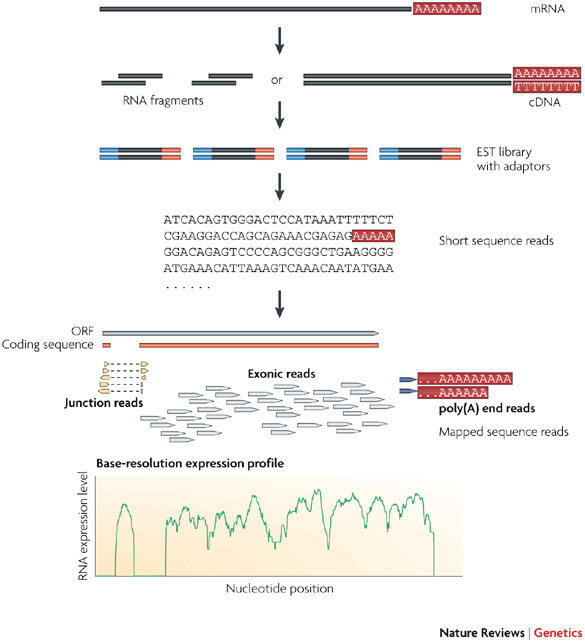
\includegraphics[width=\textwidth]{figures/rna-seq-experiment.jpg}
\caption[一般的 RNA-Seq 实验流程 \cite{wang2009rna}]{一般的 RNA-Seq 实验流程 \cite{wang2009rna}: 
长的 RNA 首先被打断成为 cDNA 库, 然后通过测序得到短的读段。
然后这些读段被比对到基因组参考序列上。}
\label{intro-rna-seq-ex}
\end{figure}

\begin{figure}[!t]
\centering
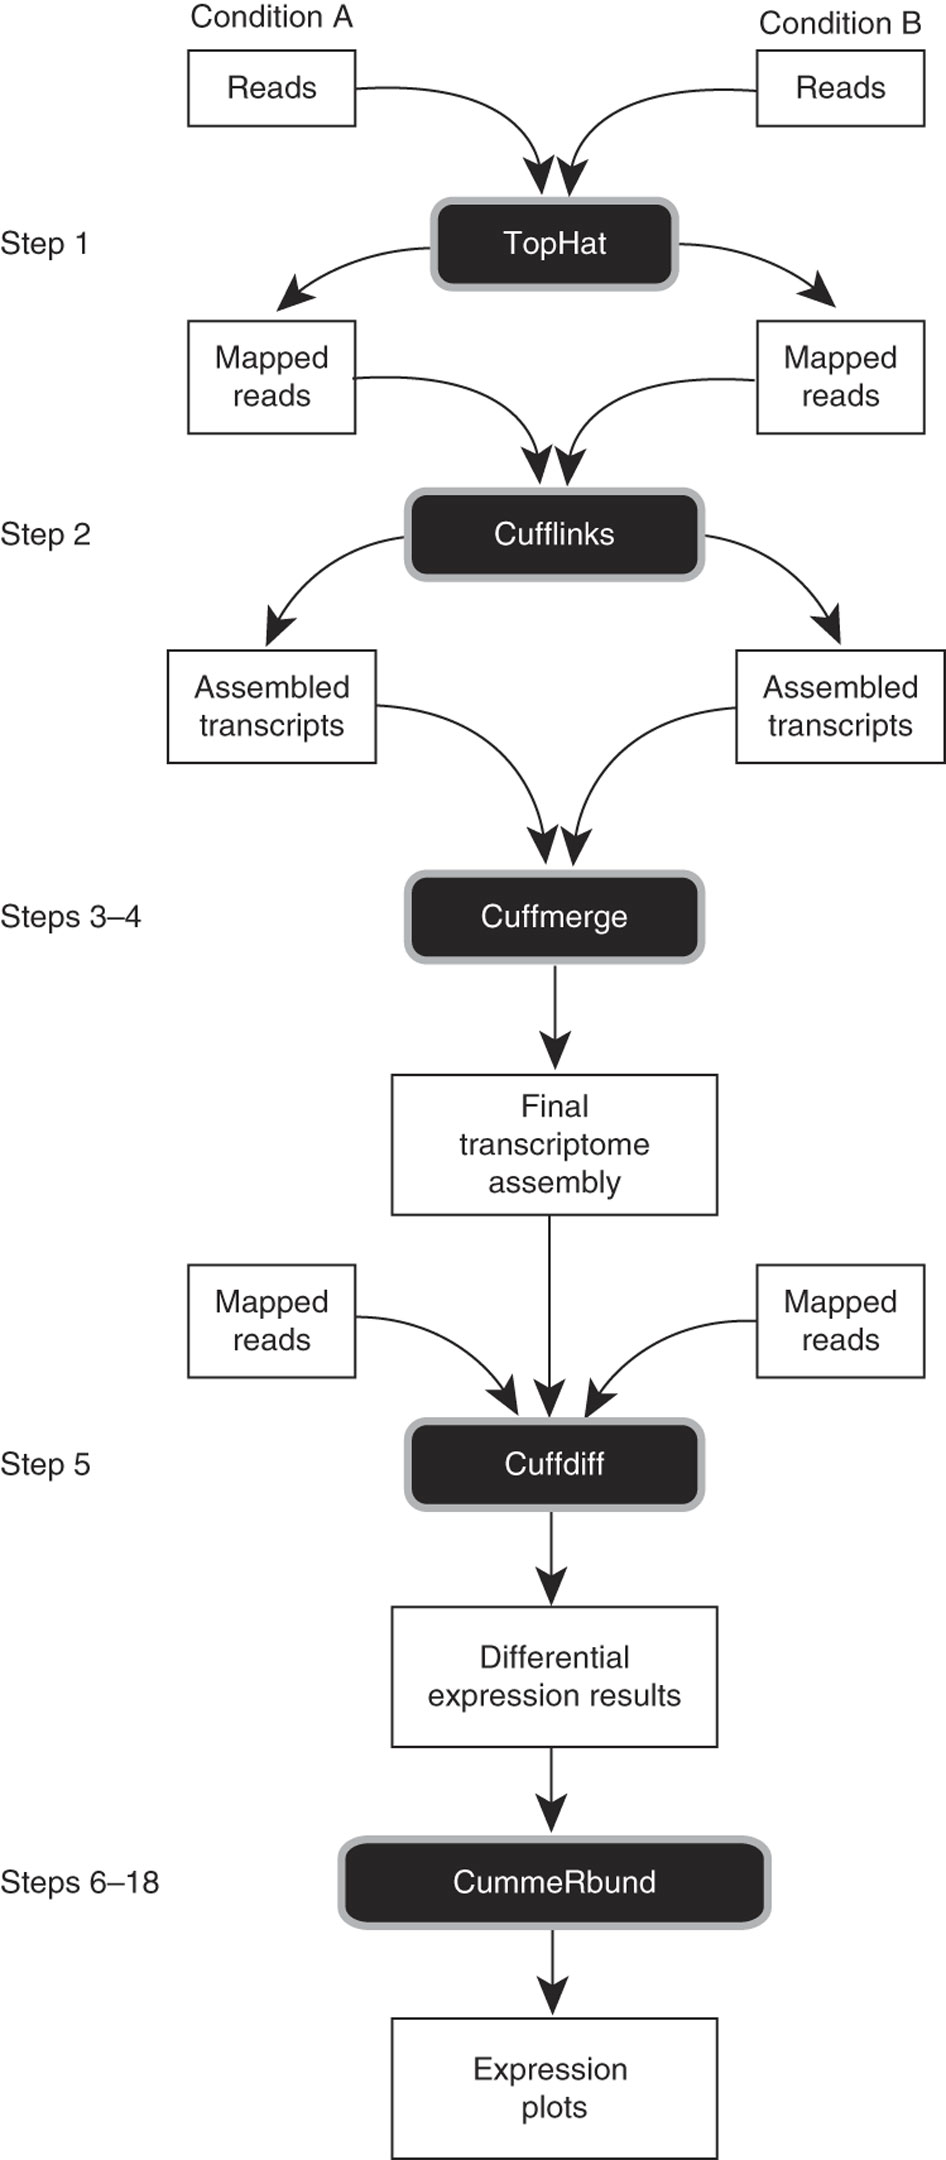
\includegraphics[height=0.85\textheight]{figures/tuxedo-protocol-tophat-cufflinks.jpg}
\caption[一般的通过 TopHat \cite {trapnell2009tophat} 和 Cufflinks 
\cite{cufflinks.2010} 分析 RNA-Seq 数据的流程 \cite{trapnell2012differential}]
{一般的通过 TopHat \cite {trapnell2009tophat} 和 Cufflinks 
\cite{cufflinks.2010} 分析 RNA-Seq 数据的流程 \cite{trapnell2012differential}: 
在一个有两种不同的条件的实验中, 读段首先被 TopHat 比对到基因组参考序列上, 
然后 Cufflinks 根据 TopHat 的比对结果组装转录本, 并且估计每一个转录本的表达量, 
最后对两个不同的条件做基因差异表达分析。}
\label{intro-rna-seq-anal}
\end{figure}

\section{RNA-Seq 数据分析方法简介}
RNA-Seq 通常直接用于发现新的剪切异构体 
\cite{merkin2012evolutionary, wang2010novo, roberts2011identification, wang2010mapsplice}, 
研究 RNA 序列的对于生物的调控作用 \cite{van2011xuts}
以及比较不同条件下转录组不同的构成 \cite{trapnell2012differential}
等生物问题的研究。
同时, RNA-Seq 数据还未研究其他生物问题提供了宝贵的原始数据, 
例如对于生物系统中的网络的研究 \cite{shalek2013single,sinicropi2012whole}。 

为了能够通过 RNA-Seq 数据对生物问题有深入的研究, 
我们通常会对 RNA-Seq 数据用这些方法进行处理:
\begin{itemize}
\item 序列比对 (sequence alignment): 将 RNA-Seq 读段找到其在基因组中的位置

\item 序列拼装: 
直接将 RNA-Seq 读段拼装成原转录组的各转录本。 若拼装时不依赖已知的参考序列, 
则成为 \textit{de novo} 拼装 (\textit{de novo} assembly) 

\item 转录本的表达量估计: 用一定的单位表示每个被测样本中转录组里每个转录本的含量, 
用于在不同的样本之间进行比较

\item 辨识同一个基因的剪切异构体 (真核生物 RNA-Seq 数据): 真核生物中由于选择性剪切同一个基因会产生多个剪切异构体, 
通过 RNA-Seq 数据在一定条件下可以辨识出一个基因的不同的剪切异构体
\end{itemize}

\subsection{序列比对}
经典的序列比对算法包括 Smith-Waterman 算法 \cite{SmithWaterman1981} 和 Needleman-Wunsch 算法 \cite{needleman1970general}。 
但是由于 Smith-Waterman 算法和 Needleman-Wunsch 算法复杂度偏高, 它们不适用于大规模的数据。 
目前人们一般采用一些启发式的方法进行序列比对 \cite{isaev2004introduction}。 
对于将 RNA-Seq 读段比对到其在基因组中的位置, 目前比较常用的工具是 
BLAT \cite{kent2002blat}
和 TopHat \cite{trapnell2009tophat}。

\subsection{序列拼装}
序列拼装是生物信息学和计算生物学中一个经典的问题, 
其目的是通过测序的读段恢复出原始的生物序列。 对于序列拼装, 目前人们主要采用 
OLC (overlap-layout-consensus) \cite{greenphrap, bonfield1995new, 
kececioglu1995combinatorial, myers1995toward, huang1999cap3}
和 de Bruijn 图 \cite{pevzner2001eulerian} 
这两种常用的策略。

目前对于 RNA-Seq 数据的拼装主常用的工具是 
Cufflinks \cite{cufflinks.2010} 和 Trinity \cite{grabherr2011full}。
其中 Cufflinks 拼装序列时使用的是 OLC 策略 (图 \ref{intro-cufflinks-assembly}), 
而 Trinity \cite{grabherr2011full} 拼装序列时使用的是 
de Bruijn 图策略 (图 \ref{intro-trinity-assembly})。

\begin{figure}[!t]
\centering
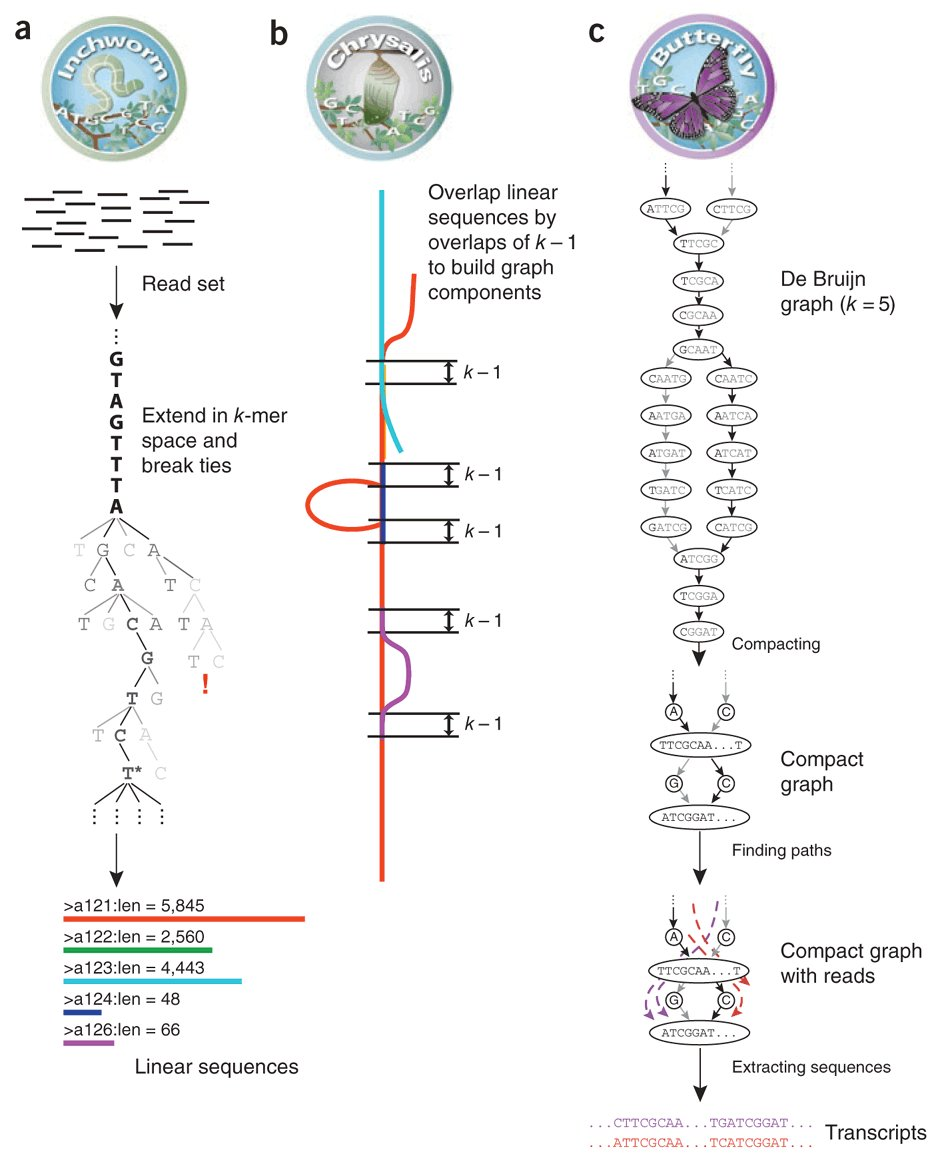
\includegraphics[width=\textwidth]{figures/trinity-assembly.jpg}
\caption[Trinity 拼装策略 \cite{grabherr2011full}]
{Trinity 拼装策略 \cite{grabherr2011full}: Trinity 拼装序列时使用的是 
de Bruijn 图策略}
\label{intro-trinity-assembly}
\end{figure}

\subsection{转录本的表达量估计}
通过量化转录组中各转录本, 从实验数据中估计其表达量, 
我们可以对生物系统中的结构和过程有更好的量化的认识。 
RNA-Seq 技术的发展对于转录本表达量的估计有很大的帮助。 
在 RNA-Seq 实验中, 
通常使用 RPKM (reads per kilobase per million reads sequenced) 
\cite{mortazavi2008mapping} 作为一个转录本表达量的单位。 
目前在 RNA-Seq 实验中通常使用的转录本表达量估计的工具是 
Cufflinks \cite{cufflinks.2010} (图 \ref{intro-cufflinks-abundance})
和 RSEM \cite{li2011rsem}。

\begin{figure}[!t]
\centering
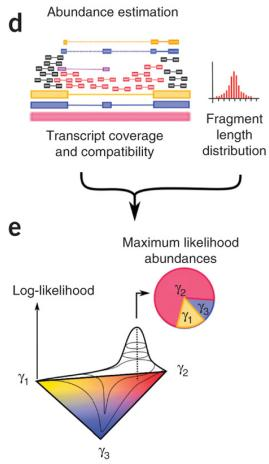
\includegraphics[height=0.5\textheight]{figures/cufflinks-abundance.jpg}
\caption[Cufflinks 对转录本的表达量的估计 \cite{cufflinks.2010}]
{Cufflinks 对转录本的表达量的估计 \cite{cufflinks.2010}: 
Cufflinks 使用一个多项式模型通过最大似然对转录本的表达量进行估计}
\label{intro-cufflinks-abundance}
\end{figure}

\subsection{辨识同一个基因的剪切异构体 (真核生物 RNA-Seq 数据)}
经过多年的研究, 人们认识到真核生物的同一个基因会有多个剪切异构体 
\cite{gilbert1978genes, rosenfeld1982calcitonin, early1980two, 
citeulike:447573, modrek2002genomic}。 
RNA-Seq 技术的发展大大促进了人们对于真核生物中选择性剪切的认识, 
因为 RNA-Seq 数据可以较好地表现出来真核生物中的选择性剪切的现象。 
目前在真核生物相关的 RNA-Seq 实验中通常使用的用于辨识同一个基因的剪切异构体的工具是 
Cufflinks \cite{cufflinks.2010} (图 \ref{intro-cufflinks-assembly})。

\begin{figure}[!t]
\centering
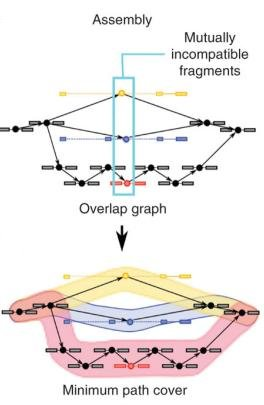
\includegraphics[height=0.5\textheight]{figures/cufflinks-assembly.jpg}
\caption[Cufflinks 序列拼装策略和对同一个基因的剪切异构体的辨识 \cite{cufflinks.2010}]
{Cufflinks 序列拼装策略和对同一个基因的剪切异构体的辨识 \cite{cufflinks.2010}: 
Cufflinks 拼装序列时使用的是 OLC 策略。
另外,Cufflinks 通过在读段位置关系构成的图中寻找一个最小路径覆盖来辨识一个基因的剪切异构体。}
\label{intro-cufflinks-assembly}
\end{figure}


\section{现有基于 RNA-Seq 数据的转录本表达量估计和剪切异构体辨识方法 (真核生物 RNA-Seq 数据)}
\label{intro-rna-seq-tools-summary}

\subsection{RNA-Seq 数据定量分析的一般模型}
\label{rna-seq-general-model}

Pachter 在 \onlinecite{2011arXiv1104.3889P} 中对 RNA-Seq 
数据定量分析建立了一个一般的模型, 
用统计的方法对 RNA-Seq 数据进行定量分析。 在这里我们对这个模型进行介绍。 

下面是为了描述该模型所使用的一些符号, 以及一些假设: 
\begin{itemize}
\item $G$ 表示转录组中所有包含的基因所组成的集合。 

\item 所有读段构成的集合表示为 $R$, 同时所有的读段都是单端测序得到的等长读段。 
(对于双端测序数据以及不等长读段的数据的处理与这里的模型相似, 此处为了叙述简便不再赘述, 
有兴趣的读者可参考 \onlinecite{cufflinks.2010} 和 \onlinecite{2011arXiv1104.3889P}。)

\item $I_g$, $g \in G$ 表示基因 $g$ 在转录组中所有的剪切异构体组成的集合, 
$I = \bigcup_{g \in G} I_g$ 是所有的剪切异构体所构成的集合。 
此处为了方便描述, 我们也将无选择性剪切的基因所对应的转录本称作是它的剪切异构体。 

\item $\theta_i \geq 0$, $i \in I$ 是剪切异构体 $i$ 的表达量, 
它们满足 $\sum_{i \in I} \theta_i = 1$。 记 $\theta_I = \{\theta_i | i \in I\}$。
在该模型下, 此处定义的表达量和实际中 RPKM 表达的表达量成正比 \cite{cufflinks.2010}。

\item $q(p, i)$ 表示对于一个剪切异构体 $i \in I$, 
来自 $i$ 的一个读段的起始位置 (5' 段) 是 $p$ 的概率。
对于给定的一个剪切异构体 $i$, 
$\sum_{p \in \{ \text{所有读段起始位置} \}} q(p, i) = 1$。
对于处理实际 RNA-Seq 数据中遇到的读段分布不均匀的问题我们可以通过调整 $q(p,i)$ 
以改进方法的准确性 \cite{roberts2011improving}。

\item 当给定一个剪切异构体 $i$ 和它上面一个读段的起始位置 $p$ 时, 
$q(p, i)$ 是已知的。

\item 一个读段 $r \in R$ 可以是来自多个 $I$ 中的剪切异构体, 
但是给定一个剪切异构体 $i$, 
用序列比对的方法将 $r$ 比对到 $i$ 上的所有位置是唯一的。 
(对于基因序列的分析表明这样一个假设是合理的 \cite{peng2011t}。) 

\item 对于一个读段 $r$ 和一个剪切异构体 $i$, 定义 $a_{ri}$: 
\[
a_{ri} = \begin{cases}
0 & \text{当 $r$ 不能比对到 $i$ 上时} \\
q(\text{$r$ 比对到 $i$ 上的起始位置},i) & \text{当 $r$ 能比对到 $i$ 上时} \end{cases}
\]

\item 对于每一个读段 $r \in R$, 
都存在一个剪切异构体 $i \in I$ 使得 $r$ 是可以由 $i$ 产生的一个读段。 

\item 所有的读段都是独立的。 
\end{itemize}
由以上我们给出到观察到所有读段 $R$ 的似然函数 \cite{2011arXiv1104.3889P}: 
\begin{equation}
\label{rna-seq-general-likelihood}
L(R) = \prod_{r \in R} (\sum_{i \in I} a_{ri} \theta_i)
\end{equation}

\subsection{转录本表达量估计和剪切异构体辨识}
在已知所有剪切异构体的集合 $I$ 时, 通过式 \eqref{rna-seq-general-likelihood} 中的似然函数, 
我们可以对各剪切异构体的表达量进行估计。 

当我们不知道剪切异构体的集合 $I$ 时, 
我们可以通过过优化通过式 \eqref{rna-seq-general-likelihood} 中的似然函数, 
或者其他的目标函数, 在进行剪切异构体集合 $I$ 的辨识的同时对各转录本的表达量进行估计 
\cite{xing2006expectation}。 
已发表的方法包括 NSMAP \cite{nsmap.21575225}, 
IsoLasso \cite{isolasso.recomb}, 
CEM \cite{Li15112012}, 
iReckon \cite{Mezlini29112012}, 
SLIDE \cite{Li13122011}, 和 
Montebello \cite{Hiller.Montebello}。

下面我们对若干已发表的通过 RNA-Seq 数据进行转录本表达量估计和剪切异构体辨识的工具进行介绍。 

\subsubsection{Cufflinks}
Cufflinks 对于剪切异构体的辨识和转录本表达量的估计如图 \ref{intro-cufflinks-assembly} 
和图 \ref{intro-cufflinks-abundance} 所示。 
Cufflinks 是分开处理剪切异构体的辨识和转录本表达量的估计这两个流程的。 
对于剪切异构体的辨识, Cufflinks 在 读段所构成的剪切图 
(splicing graph) \cite{Heber01072002} 寻找一个最小的路径覆盖, 
但是 Cufflinks 并不是直接在剪切图上进行操作的。 
Cufflinks 通过在读段之间定义一个序, 
并且在这个序构成的二分图上计算最小花费最大匹配来构成所求的最小路径覆盖。 
在定义该二分图各边的权重时, Cufflinks 采用了 Wang et al. 在 \onlinecite{wang2008alternative} 
中的方法启发式地定义权重。

\subsubsection{NSMAP, CEM, iReckon, 和 Montebello}
\label{intro-nsmap-cem-ireckon-montebllo}

NSMAP, CEM, iReckon, 和 Montebello 这 4 个工具是同时进行剪切异构体的辨识和转录本表达量的估计的。 
由于一个基因可能的剪切异构体的个数相当的多, NSMAP, CEM, iReckon, 和 Montebello 
采用了带惩罚项的似然函数进行剪切异构体的辨识和转录本表达量的估计。 
其具体做法是对式 \eqref{rna-seq-general-likelihood} 中的似然函数增加一个惩罚项, 
变为求剪切异构体的集合 $I$ 和它们的表达量 $\theta_I$ 使得
\begin{equation}
e^{-\Phi} L(R) = 
e^{-\Phi}\prod_{r \in R} (\sum_{i \in I} a_{ri} \theta_i)
\end{equation}
最大化, 其中 $\Phi \geq 0$ 是一个惩罚项, 可以使用 BIC (Bayesian information criterio) \cite{BIC.Schwarz_1978}  
($\Phi = \frac{\sum_{i \in I, \theta_i\neq 0} 1}{2} \log |R|$) 等方法。

NSMAP 和 iReckon 均使用的是 Lasso, 
而 CEM 则使用了一个 Dirichlet 分布作为先验概率。
NSMAP, CEM, 和 iReckon 在计算时采用的策略均是枚举所有剪切异构体集合 $I$ 中的可能的剪切异构体。 
由于一个基因可能的剪切异构体的个数是随它的外显子的个数的增长按指数规律增长的, 
所以 NSMAP, CEM, 和 iReckon 在计算时无法处理外显子较多的基因。 
Montebello 则是采用一个 MCMC (Markov chian Monte Carlo) \cite{robert2004monte} 的策略, 
在计算的过程中避免了枚举一个基因所有可能的剪切异构体。 

\subsubsection{IsoLasso 和 SLIDE}
IsoLasso 和 SLIDE 也是同时进行剪切异构体的辨识和转录本表达量的估计的。 
IsoLasso 和 SLIDE 采用的策略与 \ref{intro-nsmap-cem-ireckon-montebllo} 
中提到的若干工具相似, 但是 IsoLasso 和 SLIDE 并不是对式 
\eqref{rna-seq-general-likelihood} 中的似然函数进行最大化。 
这两个工具均通过将一个基因按该基因的每个外显子分为若干个区域, 
对每个区域计算读段的覆盖 (coverage), 
并根据此通过线性回归同时进行剪切异构体的辨识和转录本表达量的估计。 
这里对 IsoLasso 和 SLIDE 中所用的数学模型进行简单的介绍。 
通过 RNA-Seq 数据我们可以计算得每一个基因中的每一个外显子的覆盖 $c$, 
IsoLasso 和 SLIDE 均假设该外显子的覆盖 $c$ 是所有包含该外显子的剪切异构体的表达量之和, 
即在理想情况下应有
\begin{equation}
\label{outline-isolasso-slide}
c = \epsilon + \sum_{i \in \text{所有包含该外显子的剪切异构体}} e_i
\end{equation}
其中 $e_i$ 是剪切异构体 $i$ 的表达量 (这里的 $e_i$ 与之前所描述的 $\theta_i$ 不同), 
$\epsilon$ 是一个期望 $\operatorname[E] = 0$ 的噪声。 
IsoLasso 和 SLIDE 对目前转录组中所有的基因所包含的外显子进行类似 
式 \eqref{outline-isolasso-slide} 中的处理, 通过线性回归估计每一个剪切异构体的表达量。 
注意到通过该方法计算得的表达量值和用 RPKM 单位表达的表达量是成正比的。 
由于一个基因可能的剪切异构体的个数相当的多, 
在线性回归时 IsoLasso 和 SLIDE 均采用了 Lasso \cite{tibshirani1996regression} 用于正则化。 
与 \ref{intro-nsmap-cem-ireckon-montebllo} 中介绍的 NSMAP, CEM, 和 iReckon 类似, 
IsoLasso 和 SLIDE 在计算时采用的策略均是枚举所有剪切异构体集合 $I$ 中的可能的剪切异构体。 
由于一个基因可能的剪切异构体的个数是随它的外显子的个数的增长按指数规律增长的, 
所以 IsoLasso 和 SLIDE 在计算时无法处理外显子较多的基因。 











